\chapter{Fact-checking}
\label{chapter:fact-checking}

    \section{Problem description and goals}
    \label{section:problem-desc}
    As the motivation for this work was already given in the introduction, the following part will describe the problem. Fact-checking is an essential component in the process of news reporting, or at least it should be. Commonly interchangeably used terms \emph{fact-checking} and \emph{verification} are becoming more and more differentiated recently.~\parencite{fact-checking-vs-verification} According to~\parencite{kovach2007elements}, verification is the essence of journalism, a discipline further described as a scientific-like approach of getting the facts, which also involves verifying the source, time, location and other circumstances. Fact-checking on the other hand is more specific application of verification process focused on evaluating the veracity of a claim in some context.
    % https://www.aclweb.org/anthology/C18-1283.pdf
    
    % zahrnout obrazek demagog?
    \begin{figure}[ht]
        \label{fig:demagog}
        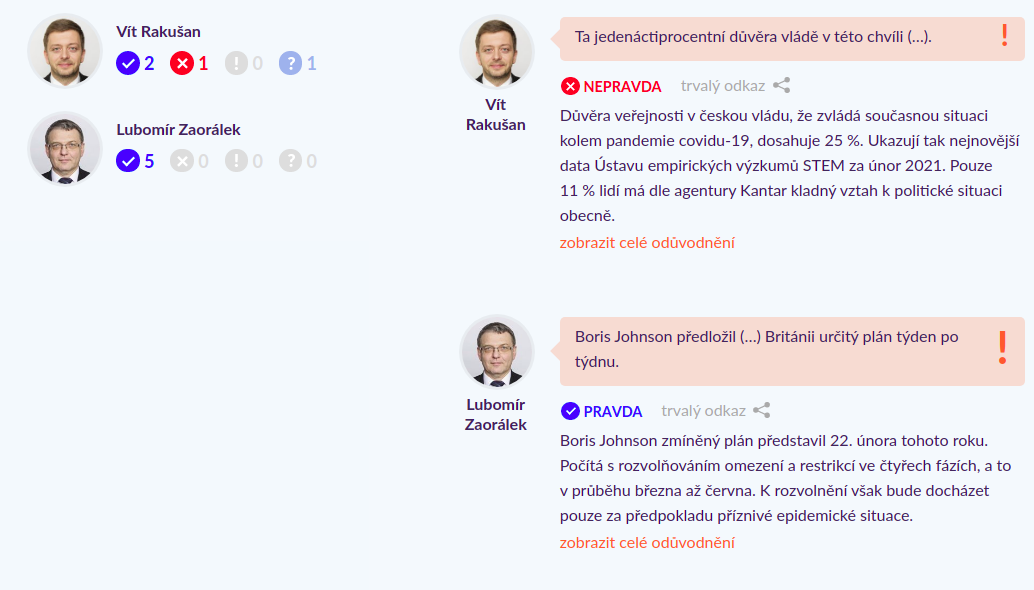
\includegraphics[width=0.9\linewidth]{demagog.png}
        \centering
        \caption[Demagog fact-checking]{Demagog fact-checking. Source: \url{https://demagog.cz}}
    \end{figure}

    Fact-checking can be illustrated on the Czech \emph{Demagog}\footnote{\url{https://demagog.cz}} project, which is based on \emph{PolitiFact}\footnote{\url{https://www.politifact.com/}} and \emph{FactCheck.org}\footnote{\url{https://www.factcheck.org/}} projects, and which manually evaluates claims, usually from political debates and interviews. Because human claim verification is laborious, time-consuming, and mentally demanding, its full or partial automation would provide significant benefits and expand the possibilities of its use, such as verifying claim in real-time political debates. However, due to the complexity of this task, in the present it is rather a distant goal. A broader introduction to automated fact-checking is presented in~\parencite{thorne-vlachos-2018-automated}.

    We defined the fact-checking task as in the~\parencite{thorne2018fever}. Verification of text claims against the knowledge base, where the knowledge base consists of text sources. The fact-checking pipeline according to the above definition is schematized in Figure~\ref{fig:factcheck-pipeline} and it can be decomposed into several sub-problems. The first step is to find relevant documents from the collection for the given claim (document retrieval). From these relevant documents, the sentences from which the evidence is formed are then selected. Finally, the veracity of the claim is classified on the basis of formed evidence (Natural Language Inference task) . %NLI
    \begin{figure}[ht]
        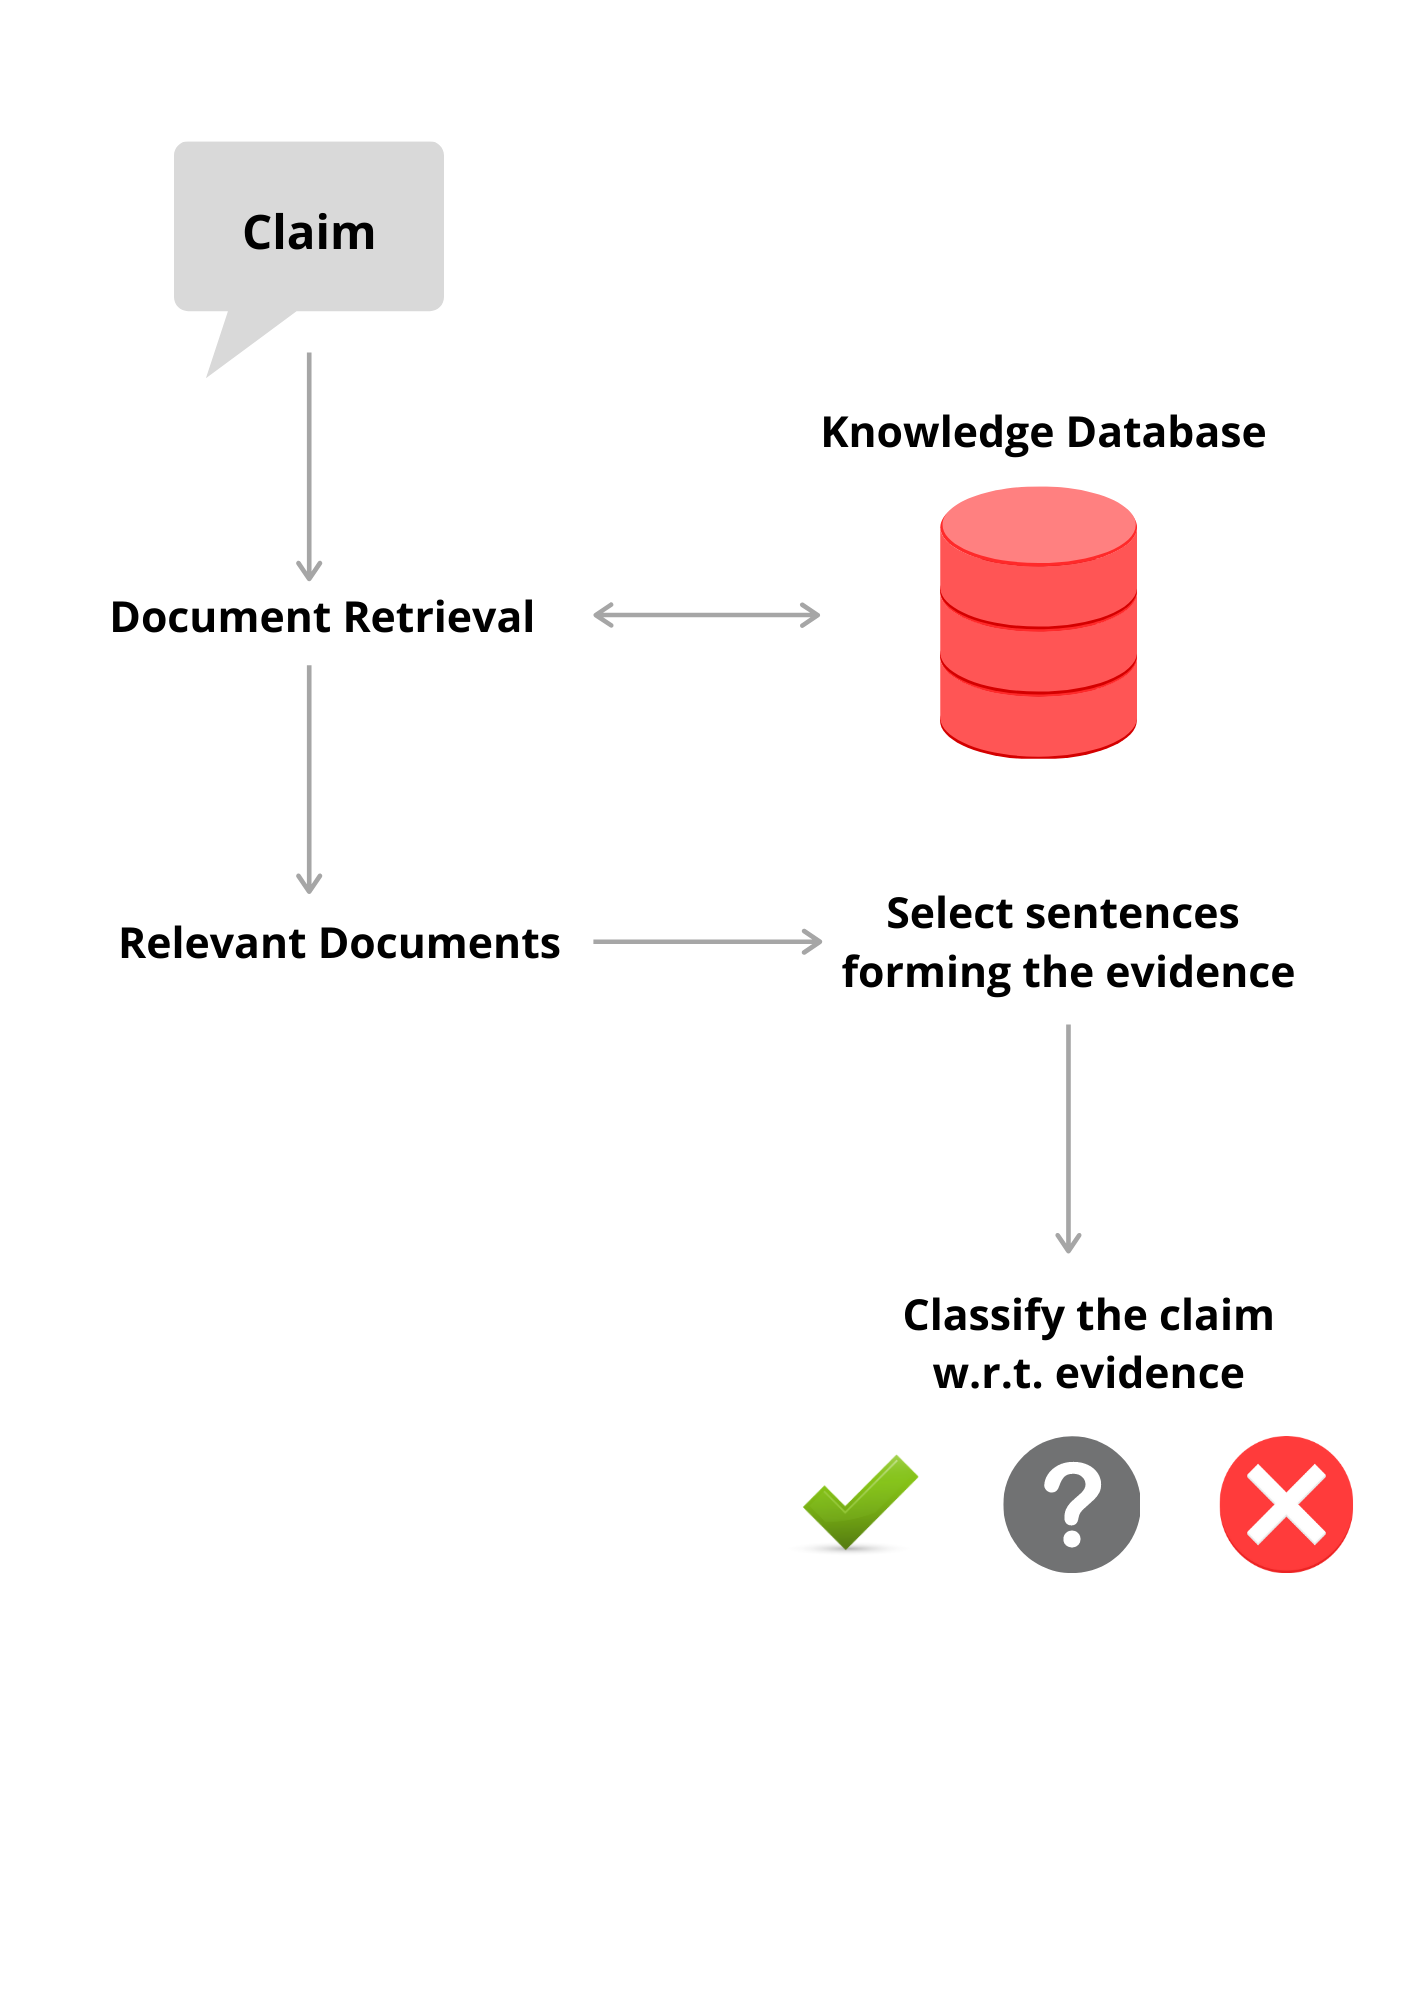
\includegraphics[width=0.6\linewidth]{fact-checking pipeline.png}
        \centering
        \caption{Fact-checking Pipeline Scheme}
        \label{fig:factcheck-pipeline}
    \end{figure}

    The aim of this thesis is to learn about large-scale document retrieval methods, examine them and evaluate them in the context of the above fact-checking pipeline. Therefore, in this thesis I will focus mainly on this part of the pipeline. Furthermore, I will focus more on neural models in order to explore their potential use in an end-to-end fact-checking system.

\section{Related work}
\label{section:related-work}
    Automatic fact-checking has recently been gaining more and more attention both in public space and in academic literature. The creation of large-scale Fact Verification and Verification (FEVER) dataset~\parencite{thorne2018fever} played a significant role in this as previously published datasets are incomparably smaller. The FEVER dataset defined the task of fact-checking much closer to real use-case by extending the task to an open domain, similarly to question-answering (QA) open-domain task in~\parencite{chen2017reading-drqa}. However, the questions usually contain some kind of clue to help you find the answer. This may not be the case for the claim whose factuality we want to verify, so finding the necessary evidence is more challenging.
    
    With the publication of the FEVER dataset, the authors also called for a submissions in shared task of claim verification using Wikipedia abstracts (first paragraph of each Wikipedia article containing high-level information) as knowledge database. The majority of submitted works followed the pipeline designed in the~\parencite{thorne2018fever} and regarding document retrieval the highest-recall solutions extracted noun phrases or named entities from the claim and used them as query in Wikipedia search API~\parencite{hanselowski-etal-2018-ukp, thorne2018fact}. In 2019, additional tasks were added to improve the resilience of systems. In the first task added, participants were asked to design a system that would generate adversarial examples that would be misclassified. In the second added task, the goal was to use these adversarial examples to create a more resilient system and improve classification performance. However, in terms of document retrieval, there was no significant change compared to the previous year~\parencite{thorne-etal-2019-fever2}. 
    %A similar approach to DR has been applied also here~\parencite{nadeem-etal-2019-fakta}, where 
    
    As far as the Czech language is concerned, we are not aware of any Czech dataset or fact-checking system, except for the dataset presented here~\parencite{priban-etal-2019-machine}. 
    
    This thesis is one of several works produced as part of the AI in Journalism project, which was supported by a \textbf{Transformation of Journalisms Ethics in the Advent of Artificial Intelligence (TL02000288)}\footnote{\url{https://starfos.tacr.cz/cs/project/TL02000288}} grant from the Technology Agency of the Czech Republic. Other works deal mainly with dataset production and the associated data annotation phase~\parencite{herbert-mt}; using hybrid (multi-stage) models for document retrieval~\parencite{bara-mt}; and document retrieval models supporting long inputs~\parencite{alex-mt}.
